We evaluate the proposed method on noisy graph signal inpainting tasks using both synthetic and real-world data.
The proposed method is compared with graph Laplacian regularization (GLR), graph total variation (GTV), and the sum of GLR and GTV (GLR+GTV).
In the synthetic experiments, we first examine recovery performance under spurious-edge and overestimated-weight inaccuracies, which directly induce the excessive-penalty failure mode targeted by the proposed regularizer.
We then consider a mixed-inaccuracy setting in which excessive-penalty and information-loss effects coexist.
Finally, we conduct experiments on real-world meteorological signals to assess the recovery performance when spatially constructed proxy graphs may naturally mismatch the underlying signal structure.

\subsection{Common Experimental Protocol}

We consider noisy graph signal inpainting under the observation model in~\eqref{eq:proposed_observation_model}.
Unless otherwise noted, the underlying signal $\mathbf{u}^{\ast}$ has $|\mathcal{V}|=256$ entries and is normalized to the range $[0,1]$.
The observation matrix $\mathbf{\Phi}$ is a binary masking matrix that randomly masks $40\%$ of the signal entries, and the additive Gaussian noise has standard deviation $\sigma=0.05$.

For all experiments, the edge weights of each graph used for recovery are rescaled so that their mean is equal to one before applying the compared methods.
This common normalization suppresses differences attributable merely to the global weight scale and allows the comparison to focus on the relative graph relations represented by the edge weights.
It also provides a common scale for the proxy-weighted edge differences whose magnitudes are controlled by the threshold parameter $\tau$ in the proposed regularizer.

We evaluate GLR, GTV, GLR+GTV, and the proposed method within the constrained recovery framework introduced in Section~IV-A, using identical data-fidelity and box constraints for all methods.
The radius $r$ of the data-fidelity ball $\mathcal{B}_{\mathbf{v},r}$ is set according to $r=\theta\sigma\sqrt{K}$, where $K$ is the number of observed signal entries, and the adjustment parameter is set to $\theta=0.9$.
The box constraint is set to $[0,1]^{|\mathcal{V}|}$ because the underlying signals are normalized to $[0,1]$.

All recovery problems are solved using P-PDS with the same numerical accuracy settings.
For each formulation, the stepsizes are determined using the variable-wise rule described in Section~II-C, with exact operator norms used for the corresponding linear operators.
Since $\mathbf{\Phi}$ is a binary masking matrix, its operator norm is one.
All optimization variables are initialized to zero, and the iterations are terminated when the norm of the update between consecutive iterates, measured in the inner-product space associated with P-PDS \cite{chambolle2011first}, becomes smaller than $10^{-9}$ or when the number of iterations reaches $10^{5}$.
Recovery performance is evaluated using the normalized root mean squared error (NRMSE):
\begin{equation}
\operatorname{NRMSE}
=
\frac{
\left\|
\widehat{\mathbf{u}}-\mathbf{u}^{\ast}
\right\|_2
}{
\left\|
\mathbf{u}^{\ast}
\right\|_2
}.
\label{eq:nrmse}
\end{equation}
Here, $\widehat{\mathbf{u}}$ and $\mathbf{u}^{\ast}$ denote the recovered and underlying signals, respectively, and a smaller NRMSE indicates more accurate recovery.
For each experimental condition, the reported performance is averaged over $20$ independent trials with independently generated observation masks and noise realizations.
For a given condition, the underlying signal and proxy graph are kept identical across all trials and methods.

For GLR+GTV and the proposed method, the parameter $\tau$ is selected from nine logarithmically spaced values ranging from $5\times10^{-3}$ to $50$.
For each method, we select a single common value of $\tau$ for each experiment by minimizing the NRMSE aggregated over all evaluation conditions considered in that experiment.
This selection is oracle because the NRMSE is evaluated using the underlying signals, but $\tau$ is not optimized separately for individual proxy-graph conditions.
The conditions included in the aggregation are described in the corresponding experimental subsections.
In addition, the synthetic experiments examine the sensitivity of the recovery performance to $\tau$, showing similar trends across the different inaccuracy settings.

\subsection{Experiments on Synthetic Data}

\begin{table}[t]
\centering
\caption{Settings for generating proxy-graph inaccuracies in the synthetic experiments.
The parameters $\rho$ and $\beta$ denote the affected-edge fraction and weight-modification factor, respectively.}
\label{tab:synthetic_settings}
\begin{tabular}{ccc}
\toprule
Inaccuracy & Fraction $\rho$ & Factor $\beta$ \\
\midrule
Spurious edges & 0.05, 0.10, 0.15, 0.20 & 2.0 \\
Overestimated weights & 0.10 & 1.0, 2.0, 3.0, 4.0 \\
Mixed inaccuracies & 0.02, 0.04, 0.06, 0.08 & 2.0 \\
\bottomrule
\end{tabular}
\end{table}

\begin{table*}[t]
\centering
\caption{Average NRMSEs under synthetic proxy-graph inaccuracies for three graph-construction settings.
``NI'' denotes the no-inaccuracy condition.
The best and second-best values within each graph setting and inaccuracy level are shown in bold and underlined, respectively.}
\label{tab:synthetic_nrmse}
\footnotesize
\begin{tabularx}{0.99\textwidth}{
@{}l
*{5}{Y}
@{}p{\dimexpr 2\tabcolsep + 6pt\relax}@{}
*{5}{Y}
@{}p{\dimexpr 2\tabcolsep + 6pt\relax}@{}
*{5}{Y}
@{}
}
\toprule
& \multicolumn{5}{c}{\textbf{Spurious edges} ($\rho$)}
&
& \multicolumn{5}{c}{\textbf{Overestimated weights} ($\beta$)}
&
& \multicolumn{5}{c}{\textbf{Mixed inaccuracies} ($\rho$)} \\
\cmidrule(lr){2-6}
\cmidrule(lr){8-12}
\cmidrule(lr){14-18}
Method
& NI & 0.05 & 0.10 & 0.15 & 0.20
&
& NI & 1 & 2 & 3 & 4
&
& NI & 0.02 & 0.04 & 0.06 & 0.08 \\
\midrule
\multicolumn{18}{@{}l}{\textbf{Setting I (reference): $(0.14,\,1.0)$}} \\
\addlinespace[2pt]
GLR
& 0.1290 & 0.1481 & 0.1631 & 0.1760 & \underline{0.1836}
&
& 0.1290 & 0.1311 & 0.1351 & 0.1379 & 0.1399
&
& 0.1290 & 0.1342 & 0.1484 & 0.1571 & 0.1656 \\
GTV
& \underline{0.1216} & \underline{0.1376} & \underline{0.1581} & 0.1775 & 0.1909
&
& \underline{0.1216} & 0.1253 & 0.1318 & 0.1366 & 0.1404
&
& \underline{0.1216} & \textbf{0.1259} & \underline{0.1392} & \underline{0.1534} & 0.1687 \\
GLR+GTV
& \textbf{0.1208} & 0.1405 & 0.1585 & \underline{0.1737} & \underline{0.1836}
&
& \textbf{0.1208} & \textbf{0.1240} & \underline{0.1305} & \underline{0.1356} & \underline{0.1394}
&
& \textbf{0.1208} & \underline{0.1265} & 0.1416 & 0.1538 & \underline{0.1644} \\
Proposed
& 0.1237 & \textbf{0.1318} & \textbf{0.1452} & \textbf{0.1572} & \textbf{0.1697}
&
& 0.1233 & \underline{0.1252} & \textbf{0.1282} & \textbf{0.1299} & \textbf{0.1316}
&
& 0.1237 & 0.1265 & \textbf{0.1337} & \textbf{0.1413} & \textbf{0.1510} \\
\midrule
\multicolumn{18}{@{}l}{\textbf{Setting II: $(0.16,\,1.0)$}} \\
\addlinespace[2pt]
GLR
& \underline{0.1001} & 0.1212 & 0.1361 & 0.1422 & \underline{0.1495}
&
& 0.1001 & 0.1021 & 0.1063 & \underline{0.1097} & \underline{0.1125}
&
& \underline{0.1001} & 0.1097 & 0.1232 & 0.1320 & \underline{0.1396} \\
GTV
& 0.1019 & 0.1202 & 0.1377 & 0.1508 & 0.1615
&
& 0.1019 & 0.1041 & 0.1084 & 0.1143 & 0.1179
&
& 0.1019 & 0.1083 & 0.1225 & 0.1343 & 0.1470 \\
GLR+GTV
& \textbf{0.0991} & \underline{0.1199} & \underline{0.1350} & \underline{0.1419} & 0.1497
&
& \textbf{0.0991} & \underline{0.1012} & \underline{0.1059} & 0.1099 & 0.1132
&
& \textbf{0.0986} & \underline{0.1082} & \underline{0.1219} & \underline{0.1317} & 0.1404 \\
Proposed
& 0.1010 & \textbf{0.1137} & \textbf{0.1261} & \textbf{0.1343} & \textbf{0.1438}
&
& \underline{0.0996} & \textbf{0.1010} & \textbf{0.1040} & \textbf{0.1062} & \textbf{0.1081}
&
& 0.1010 & \textbf{0.1068} & \textbf{0.1153} & \textbf{0.1250} & \textbf{0.1324} \\
\midrule
\multicolumn{18}{@{}l}{\textbf{Setting III: $(0.14,\,0.4)$}} \\
\addlinespace[2pt]
GLR
& 0.0721 & 0.1227 & 0.1524 & \underline{0.1694} & \underline{0.1773}
&
& 0.0721 & 0.0917 & 0.1007 & 0.1062 & \underline{0.1103}
&
& 0.0721 & 0.0971 & 0.1194 & \underline{0.1422} & \underline{0.1573} \\
GTV
& \underline{0.0660} & \underline{0.1109} & 0.1497 & 0.1808 & 0.1863
&
& \underline{0.0660} & \underline{0.0831} & \underline{0.0957} & 0.1097 & 0.1200
&
& \underline{0.0660} & 0.0882 & \underline{0.1100} & 0.1442 & 0.1665 \\
GLR+GTV
& \textbf{0.0620} & 0.1175 & \underline{0.1490} & 0.1698 & 0.1783
&
& \textbf{0.0620} & 0.0834 & 0.0969 & \underline{0.1054} & 0.1117
&
& \textbf{0.0619} & \underline{0.0881} & 0.1112 & 0.1423 & 0.1605 \\
Proposed
& 0.0705 & \textbf{0.0934} & \textbf{0.1126} & \textbf{0.1305} & \textbf{0.1451}
&
& 0.0705 & \textbf{0.0816} & \textbf{0.0852} & \textbf{0.0888} & \textbf{0.0907}
&
& 0.0705 & \textbf{0.0779} & \textbf{0.0949} & \textbf{0.1084} & \textbf{0.1176} \\
\bottomrule
\end{tabularx}
\end{table*}

\begin{figure*}[t]
\centering
\subfloat[Spurious edges]{
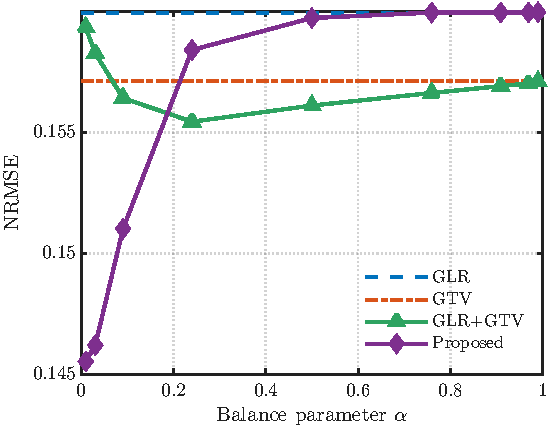
\includegraphics[width=0.31\textwidth]{images/performance_vs_balance_parameter_edge_insertion_nrmse_mean.pdf}
}
\hfill
\subfloat[Overestimated weights]{
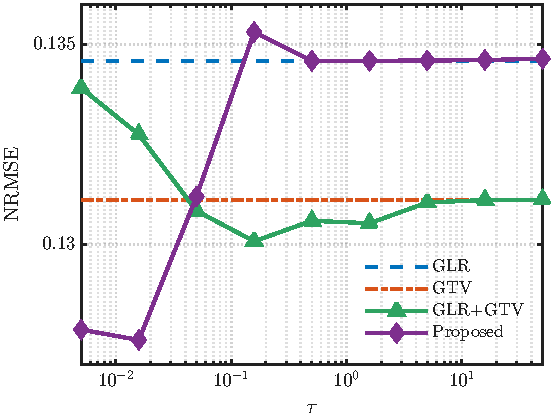
\includegraphics[width=0.31\textwidth]{images/performance_vs_balance_parameter_excessive_weights_nrmse_mean.pdf}
}
\hfill
\subfloat[Mixed inaccuracies]{
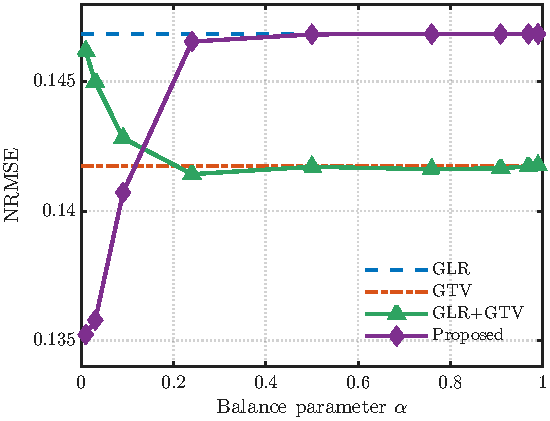
\includegraphics[width=0.31\textwidth]{images/performance_vs_balance_parameter_all_inaccuracies_nrmse_mean.pdf}
}
\caption{Average NRMSE versus the parameter $\tau$ for the reference graph setting under (a) spurious-edge, (b) overestimated-weight, and (c) mixed inaccuracies.
Each value is averaged over all tested inaccuracy levels including the no-inaccuracy condition.}
\label{fig:parameter_sensitivity}
\end{figure*}

\begin{figure*}[t]
\centering
\footnotesize
\setlength{\tabcolsep}{1pt}
\subfloat[Spurious edges]{
\begin{minipage}{0.99\textwidth}
\centering
\sbox{\fullpanelbox}{
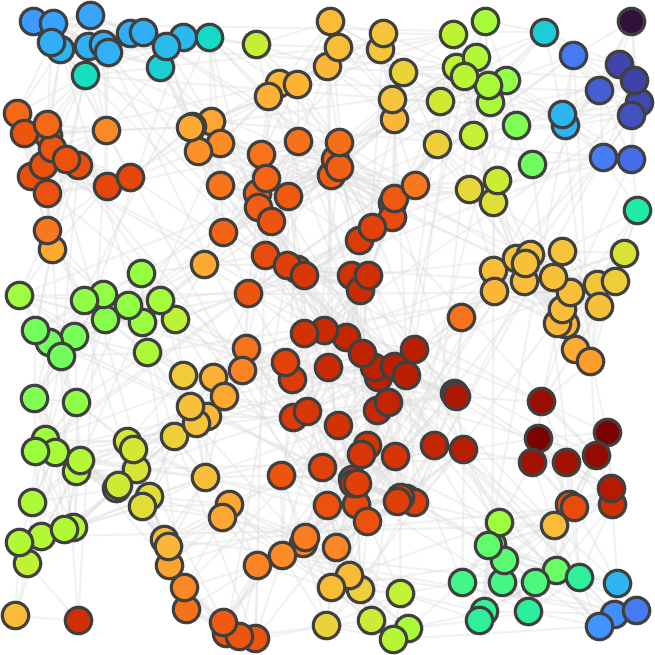
\includegraphics[width=0.15\textwidth]{images/signal_seed9_full_true.png}
}
\sbox{\targetpanelbox}{
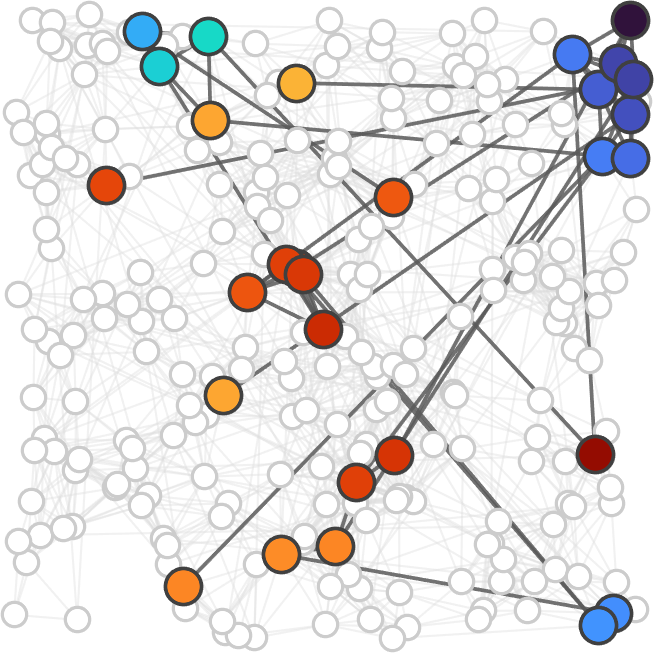
\includegraphics[width=0.15\textwidth]{images/signal_seed9_target_true.png}
}
\begin{tabular}{@{}cccccc@{\hspace{2pt}}c@{}}
\usebox{\fullpanelbox} &
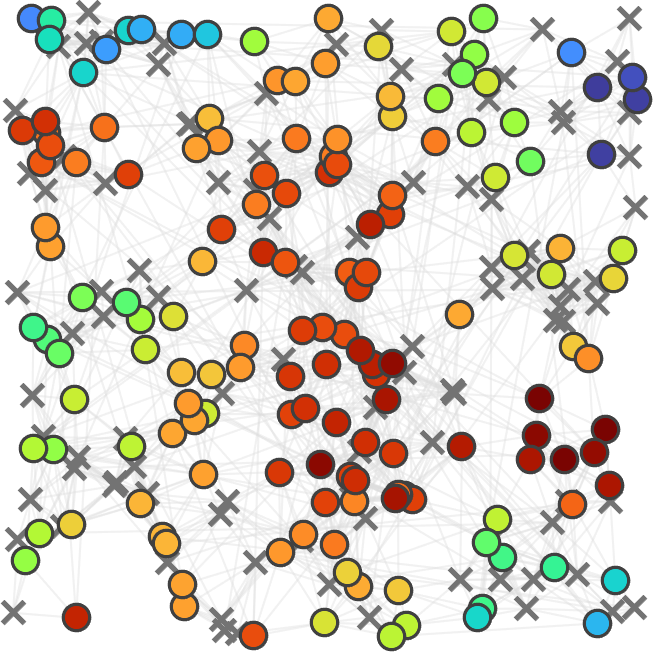
\includegraphics[width=0.15\textwidth]{images/signal_seed9_full_obs.png} &
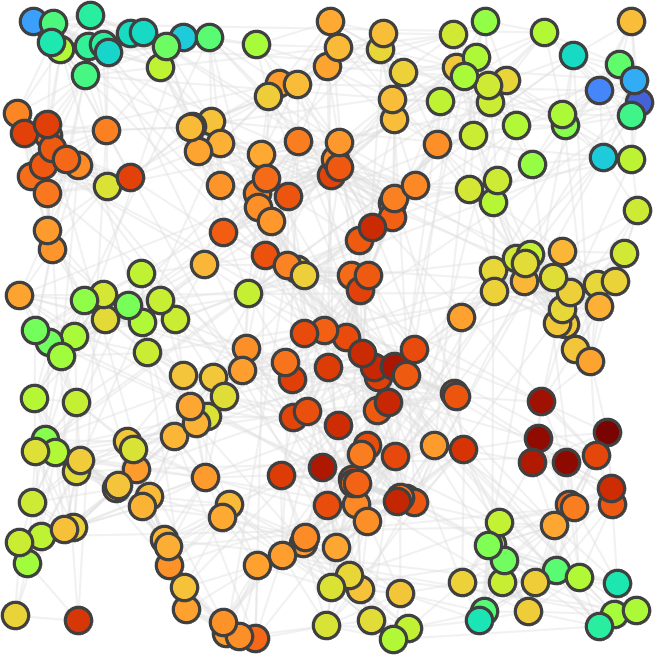
\includegraphics[width=0.15\textwidth]{images/signal_seed9_full_glr.png} &
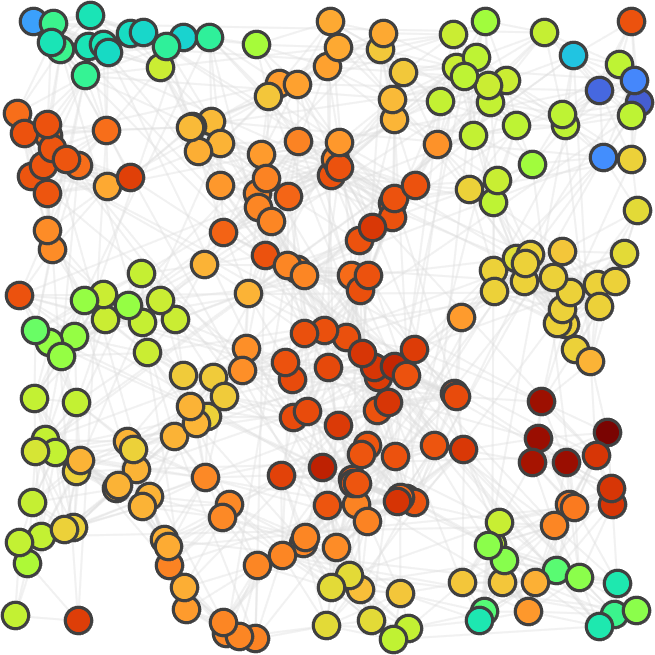
\includegraphics[width=0.15\textwidth]{images/signal_seed9_full_gtv.png} &
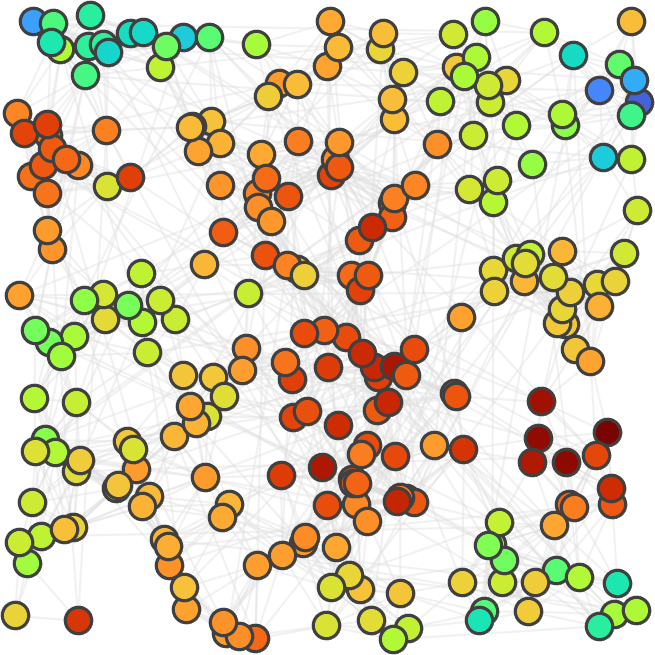
\includegraphics[width=0.15\textwidth]{images/signal_seed9_full_glr_gtv.png} &
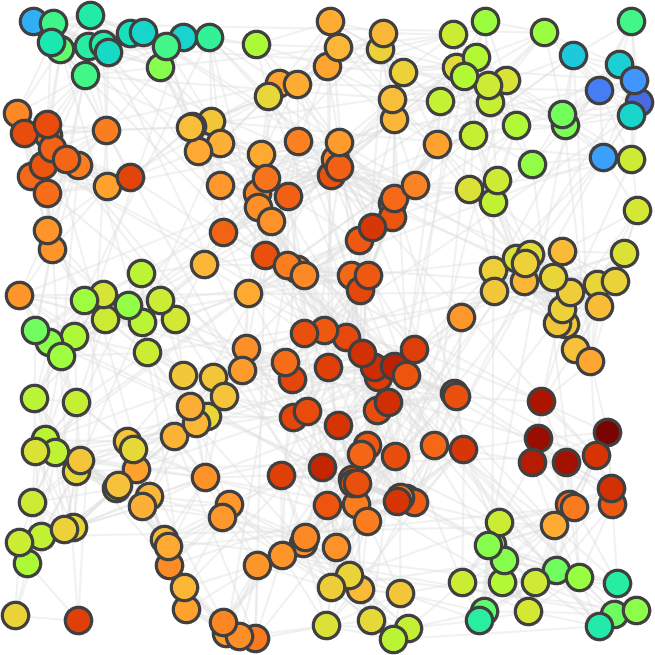
\includegraphics[width=0.15\textwidth]{images/signal_seed9_full_proposal_2.png} &
\makebox[0.035\textwidth][l]{

\includegraphics[
height=\ht\fullpanelbox,
keepaspectratio
]{images/colorbar_signal_value.pdf}
} \\
\usebox{\targetpanelbox} &
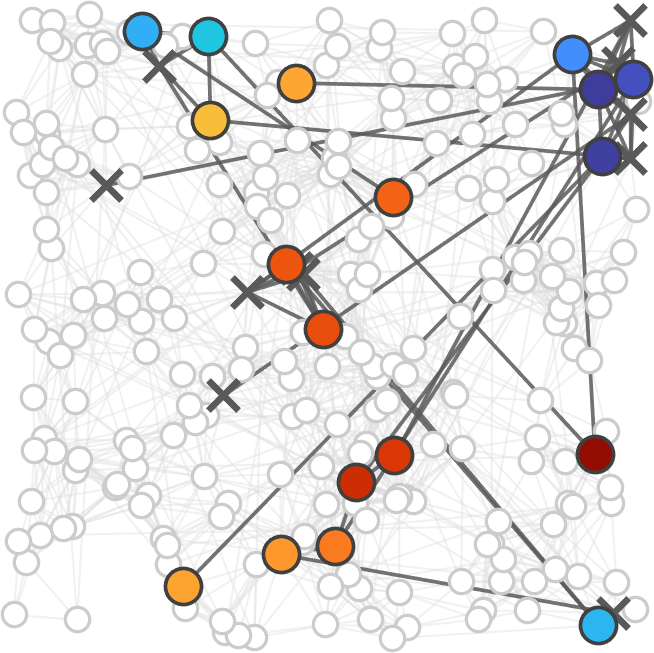
\includegraphics[width=0.15\textwidth]{images/signal_seed9_target_obs.png} &
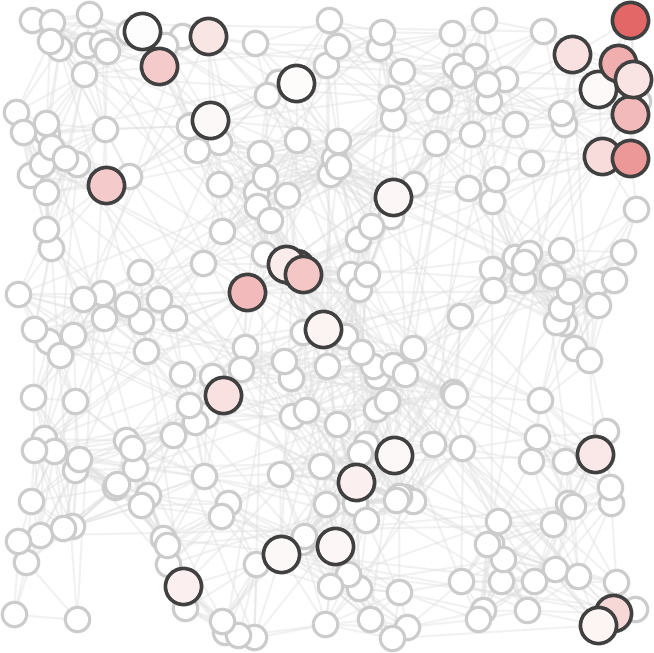
\includegraphics[width=0.15\textwidth]{images/signal_seed9_target_glr.png} &
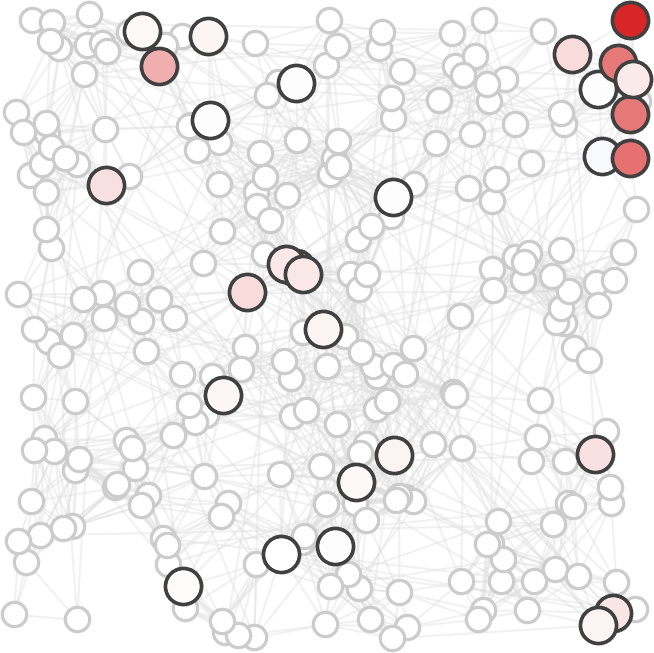
\includegraphics[width=0.15\textwidth]{images/signal_seed9_target_gtv.png} &
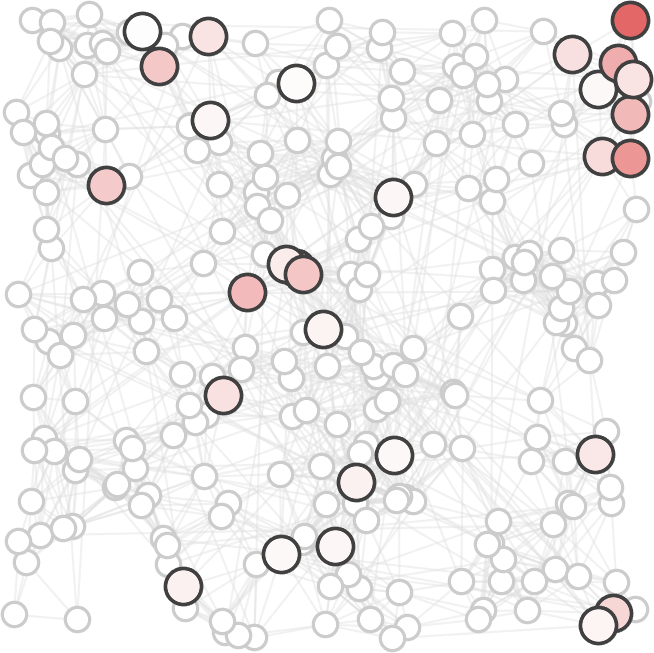
\includegraphics[width=0.15\textwidth]{images/signal_seed9_target_glr_gtv.png} &
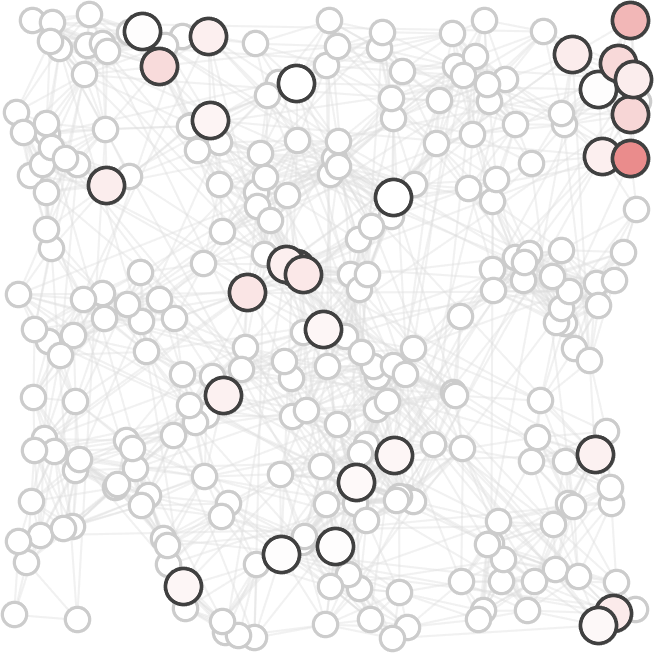
\includegraphics[width=0.15\textwidth]{images/signal_seed9_target_proposal_2.png} &
\makebox[0.035\textwidth][l]{
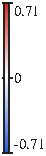
\includegraphics[
height=\ht\targetpanelbox,
keepaspectratio
]{images/colorbar_error_change_seed9.pdf}
} \\
\scriptsize\shortstack{Reference\\\phantom{NRMSE = 0.XXXX}} &
\scriptsize\shortstack{Observed\\\phantom{NRMSE = 0.XXXX}} &
\scriptsize\shortstack{GLR\\NRMSE = 0.0577} &
\scriptsize\shortstack{GTV\\NRMSE = 0.0577} &
\scriptsize\shortstack{GLR+GTV\\NRMSE = 0.0573} &
\scriptsize\shortstack{Proposed\\NRMSE = \textbf{0.0342}} &
{}
\end{tabular}
\end{minipage}
}
\par\vspace{2mm}
\subfloat[Overestimated weights]{
\begin{minipage}{0.99\textwidth}
\centering
\sbox{\fullpanelbox}{
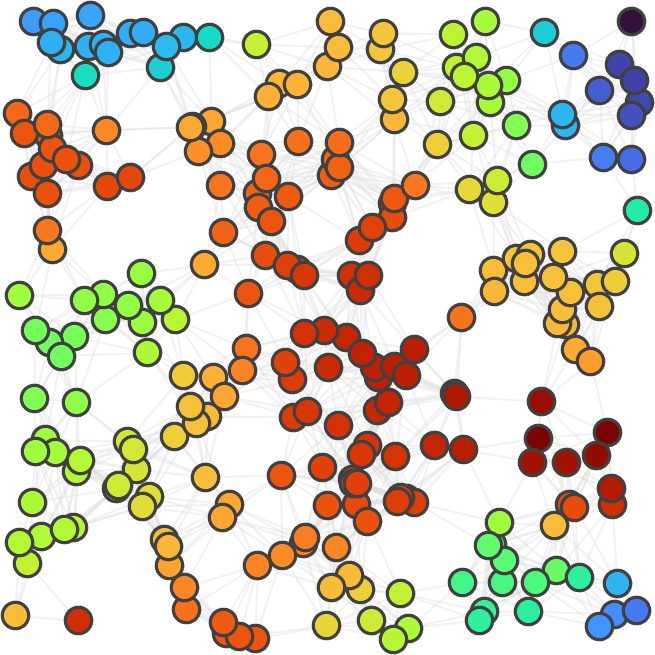
\includegraphics[width=0.15\textwidth]{images/signal_excessive_weights_seed9_full_true.png}
}
\sbox{\targetpanelbox}{
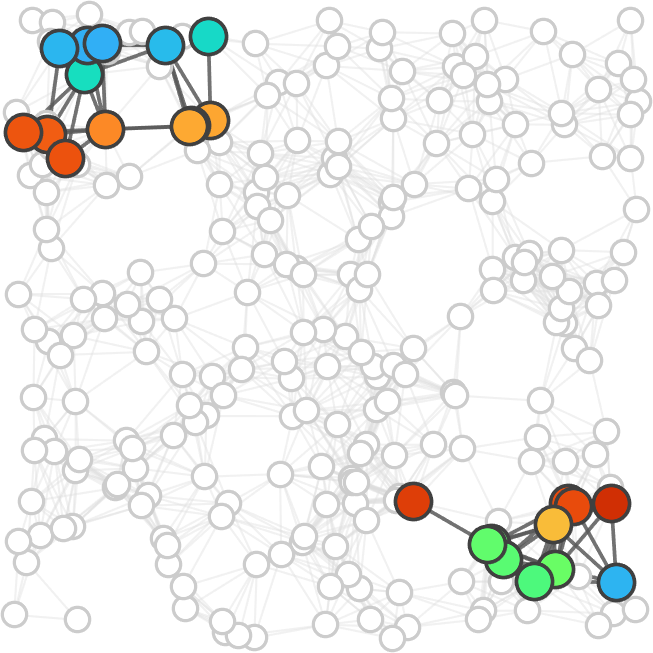
\includegraphics[width=0.15\textwidth]{images/signal_excessive_weights_seed9_target_true.png}
}
\begin{tabular}{@{}cccccc@{\hspace{2pt}}c@{}}
\usebox{\fullpanelbox} &
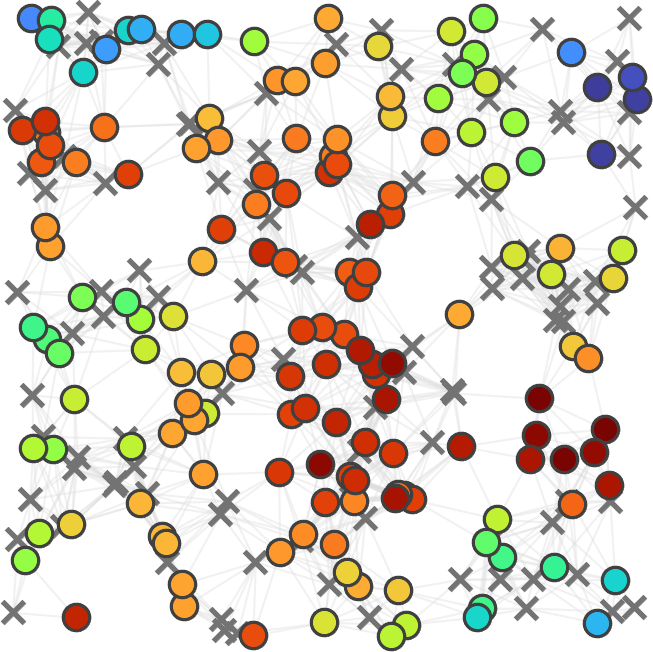
\includegraphics[width=0.15\textwidth]{images/signal_excessive_weights_seed9_full_obs.png} &
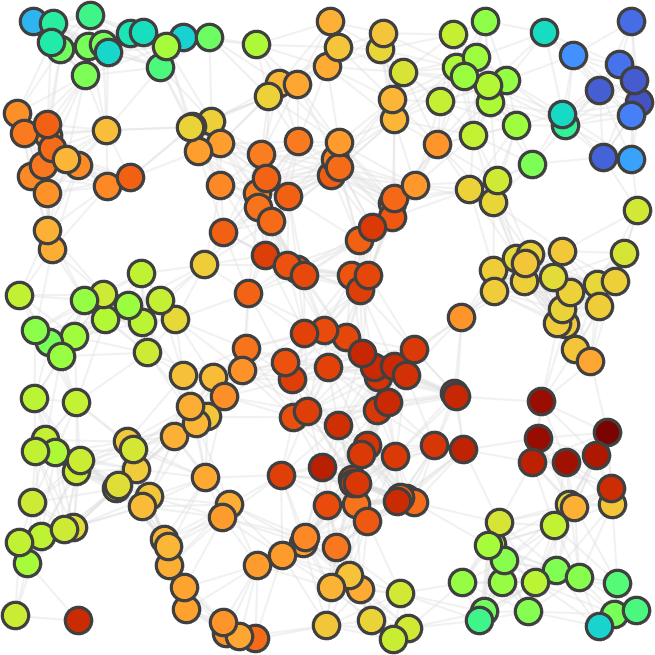
\includegraphics[width=0.15\textwidth]{images/signal_excessive_weights_seed9_full_glr.png} &
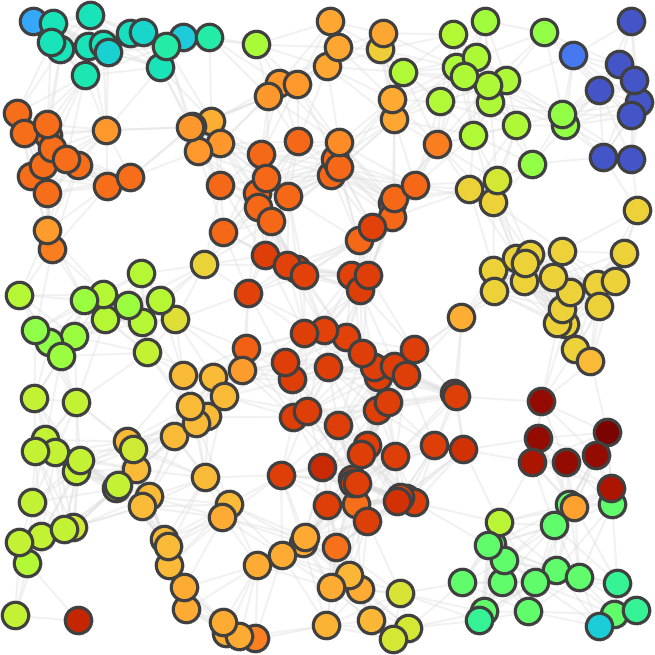
\includegraphics[width=0.15\textwidth]{images/signal_excessive_weights_seed9_full_gtv.png} &
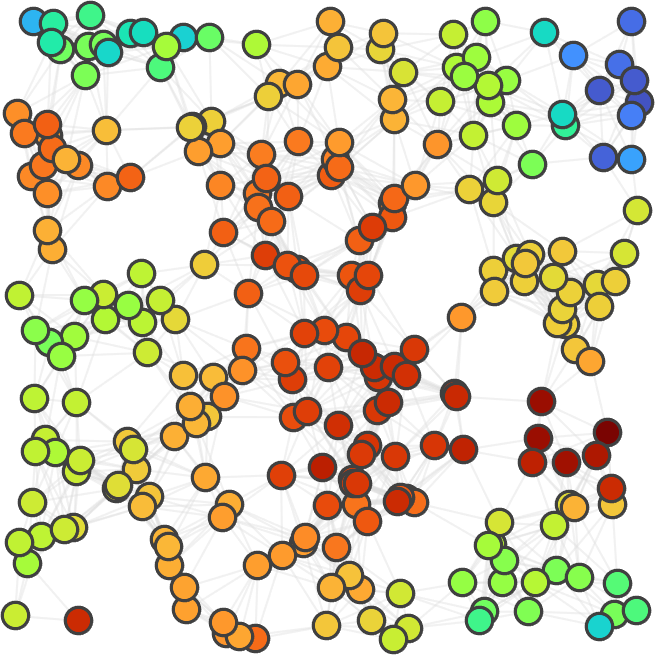
\includegraphics[width=0.15\textwidth]{images/signal_excessive_weights_seed9_full_glr_gtv.png} &
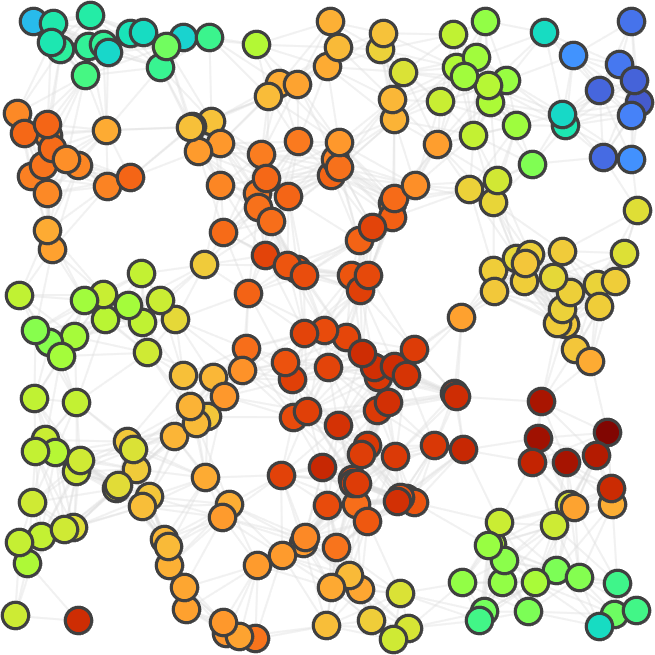
\includegraphics[width=0.15\textwidth]{images/signal_excessive_weights_seed9_full_proposal_2.png} &
\makebox[0.035\textwidth][l]{

\includegraphics[
height=\ht\fullpanelbox,
keepaspectratio
]{images/colorbar_signal_value.pdf}
} \\
\usebox{\targetpanelbox} &
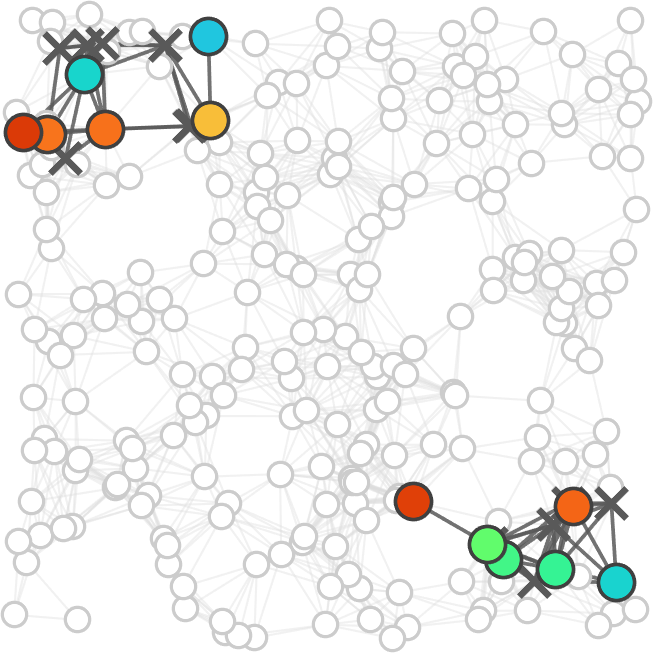
\includegraphics[width=0.15\textwidth]{images/signal_excessive_weights_seed9_target_obs.png} &
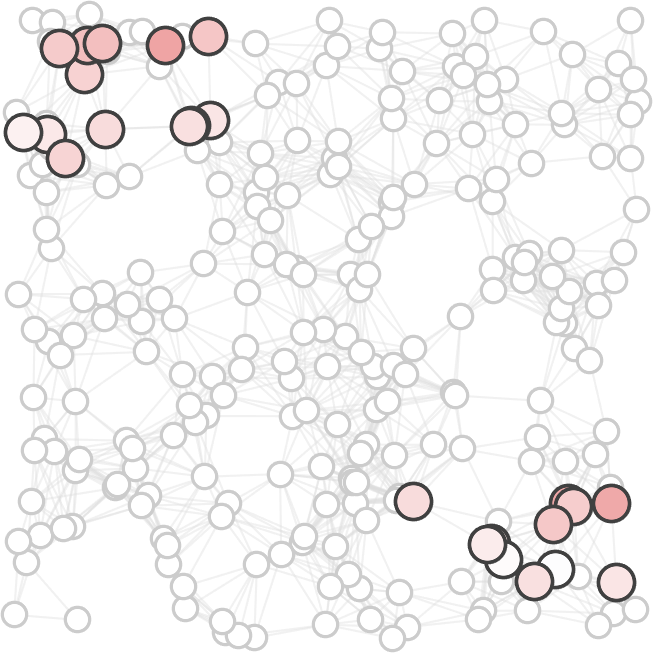
\includegraphics[width=0.15\textwidth]{images/signal_excessive_weights_seed9_target_glr.png} &
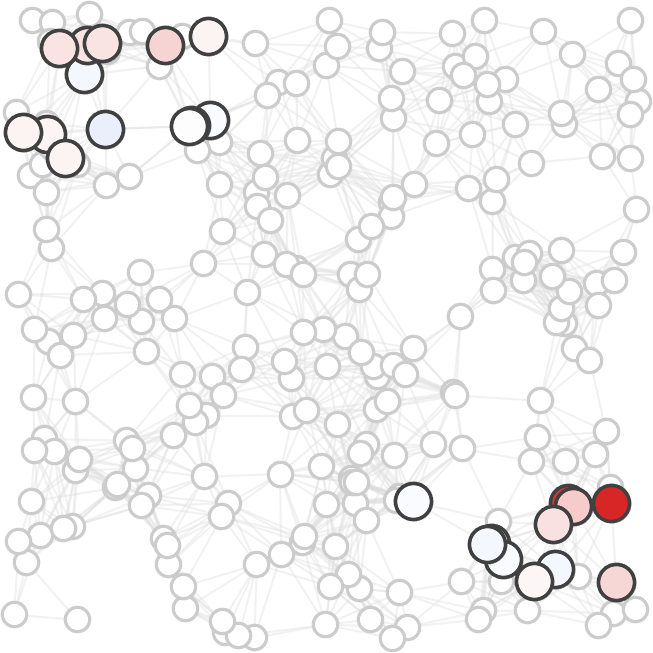
\includegraphics[width=0.15\textwidth]{images/signal_excessive_weights_seed9_target_gtv.png} &
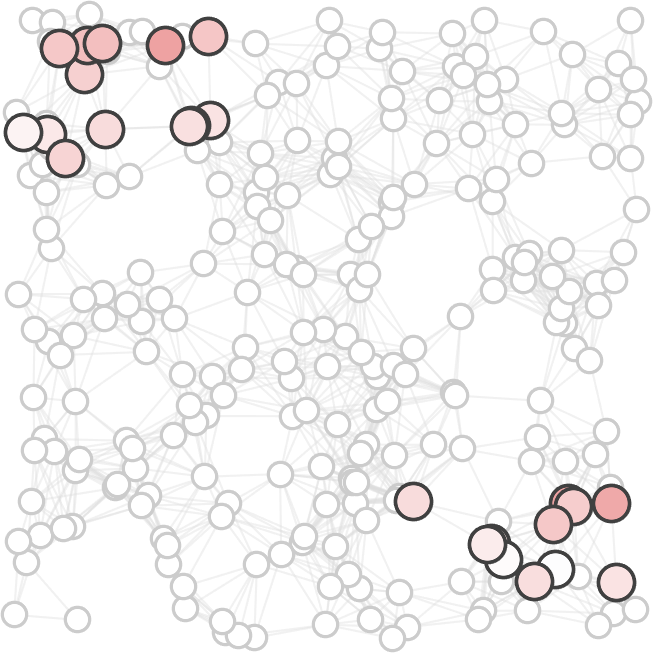
\includegraphics[width=0.15\textwidth]{images/signal_excessive_weights_seed9_target_glr_gtv.png} &
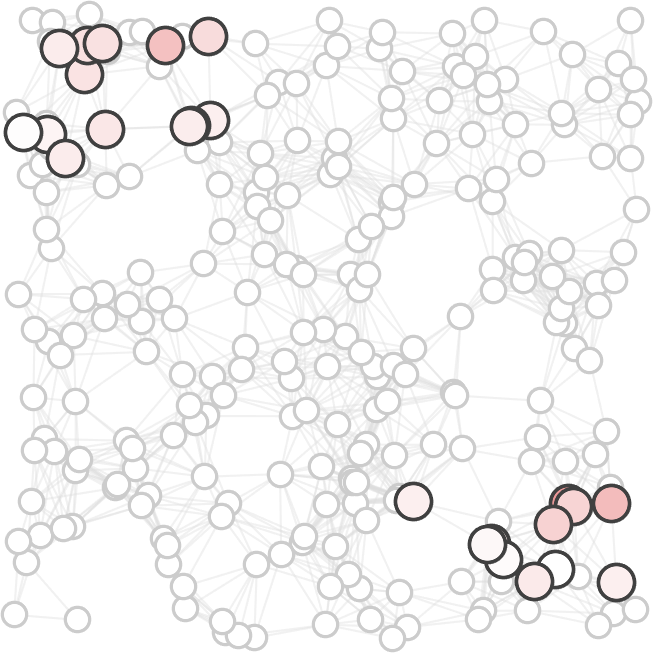
\includegraphics[width=0.15\textwidth]{images/signal_excessive_weights_seed9_target_proposal_2.png} &
\makebox[0.035\textwidth][l]{
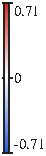
\includegraphics[
height=\ht\targetpanelbox,
keepaspectratio
]{images/colorbar_error_change_seed9.pdf}
} \\
\scriptsize\shortstack{Reference\\\phantom{NRMSE = 0.XXXX}} &
\scriptsize\shortstack{Observed\\\phantom{NRMSE = 0.XXXX}} &
\scriptsize\shortstack{GLR\\NRMSE = 0.1294} &
\scriptsize\shortstack{GTV\\NRMSE = 0.1488} &
\scriptsize\shortstack{GLR+GTV\\NRMSE = 0.1295} &
\scriptsize\shortstack{Proposed\\NRMSE = \textbf{0.0654}} &
{}
\end{tabular}
\end{minipage}
}
\caption{Qualitative recovery results with a connection radius of $0.14$ and a Gaussian-kernel standard deviation of $0.4$ under (a) spurious-edge inaccuracies with $\beta=2$ and (b) overestimated-weight inaccuracies with $\rho=0.1$.
Upper rows show the reference, observed, and recovered signals; lower rows focus on nodes incident to the top $10\%$ inaccurate edges.
Colors in the lower method panels indicate the change in absolute restoration error from NI (blue: improved; red: degraded).}
\label{fig:synthetic_qualitative}
\end{figure*}

\subsubsection{Experimental Settings}

To evaluate the proposed regularizer under controlled proxy-graph inaccuracies, we consider three types of synthetic inaccuracies: spurious edges, overestimated weights, and mixed inaccuracies.
The first two isolate the excessive-penalty failure mode targeted by the proposed regularizer, whereas the mixed setting provides a scenario in which excessive-penalty and information-loss effects coexist.

To examine whether the observed behavior depends strongly on a particular underlying graph construction, we evaluate three graph-construction settings, denoted Settings I--III.
In each setting, the underlying graph is a random geometric graph \cite{DallChristensen2002} with $256$ nodes whose locations $\{\mathbf{p}_i\}_{i=1}^{256}$ are sampled from the uniform distribution over the unit square $[0,1]^2$.
The graph topology is determined by a connection radius, and the edge weights are assigned using a Gaussian kernel.
Settings I--III use the pairs $(0.14,1.0)$, $(0.16,1.0)$, and $(0.14,0.4)$, respectively, where the first and second entries denote the connection radius and Gaussian-kernel standard deviation.

For each graph-construction setting, the underlying graph signal is generated as a random linear combination of the lowest-frequency $5\%$ of the graph Fourier components of the corresponding underlying graph.
The coefficients are independently drawn from a zero-mean Gaussian distribution with standard deviation one, and the resulting signal is normalized to the range $[0,1]$.
Proxy graphs are then generated by perturbing the topology and edge weights of the corresponding underlying graph.
The unmodified underlying graph is additionally evaluated as the no-inaccuracy (NI) reference.

The four types of proxy-graph inaccuracies used in the synthetic experiments are generated according to the following rules, where their severity is characterized by the affected-edge fraction $\rho$ and the weight-modification factor $\beta$.
Let $\mathcal{E}^{\ast}$ be the edge set of the underlying graph and let $w_{\max}$ and $w_{\min}$ denote its maximum and minimum edge weights, respectively.
Spurious-edge inaccuracies are generated by randomly selecting $\rho|\mathcal{E}^{\ast}|$ node pairs that are not connected in the underlying graph and assigning each inserted edge the weight $\beta w_{\max}$.
Missing-edge inaccuracies are generated by removing $\rho|\mathcal{E}^{\ast}|$ existing edges in descending order of their underlying weights.
Overestimated-weight inaccuracies are generated by replacing the smallest selected $\rho|\mathcal{E}^{\ast}|$ edge weights with $\beta w_{\max}$, whereas underestimated-weight inaccuracies are generated by replacing the largest selected $\rho|\mathcal{E}^{\ast}|$ edge weights with $w_{\min}/\beta$.
For the mixed-inaccuracy setting, the spurious- and missing-edge inaccuracies are introduced first, followed by the overestimated- and underestimated-weight inaccuracies on distinct remaining edges to avoid overlap among the affected edges.
The same affected-edge fraction $\rho$ is applied separately to all four inaccuracy types in the mixed setting.
The parameter values evaluated in the three inaccuracy experiments are summarized in Table~\ref{tab:synthetic_settings}.

Following the common parameter-selection protocol in Section~V-A, the reported results for each synthetic inaccuracy experiment correspond to a single common value of $\tau$ selected over all tested inaccuracy levels, rather than to values separately optimized for individual levels.

\subsubsection{Results}

Table~\ref{tab:synthetic_nrmse} summarizes the average NRMSEs under the three types of proxy-graph inaccuracies for the three graph-construction settings.
We first examine the spurious-edge and overestimated-weight experiments, which directly correspond to the excessive-penalty failure mode discussed in Section~III-A.

For spurious-edge inaccuracies, the recovery performance of all methods generally degrades as the affected-edge fraction $\rho$ increases.
However, the NRMSE of the proposed method increases more gradually than those of the comparison methods across all three graph-construction settings.
Although GTV or GLR+GTV can achieve lower NRMSE under the NI condition, the proposed method achieves the lowest NRMSE at every nonzero tested spurious-edge fraction in all three graph-construction settings.

A similar trend is observed for overestimated weights.
As $\beta$ increases, thereby strengthening the weight overestimation while keeping the affected-edge fraction fixed, the relative advantage of the proposed method becomes more pronounced.
In particular, the proposed method achieves the lowest NRMSE at the larger tested values of $\beta$ in all three graph-construction settings.

The common behavior of these two experiments is important because the inaccuracies modify different aspects of the proxy graph.
Spurious edges alter the graph topology, whereas overestimated weights preserve the topology and modify the strengths of existing graph relations.
The observed trend is therefore consistent with the mechanism developed in Section~III-B: the proposed regularizer limits the influence of excessively large proxy-weighted edge differences according to their magnitudes, rather than relying on a particular type of graph perturbation.

We next examine the mixed-inaccuracy experiment, in which excessive-penalty and information-loss effects coexist.
As the common affected-edge fraction $\rho$ increases, the NRMSE of the proposed method again increases more gradually than those of the comparison methods across the three graph-construction settings.
The proposed method achieves the lowest NRMSE at the larger tested fractions in every setting.
These results show that the benefit of magnitude-adaptive regularization is retained even when the two failure modes occur simultaneously.
The proposed method does not restore graph information removed by missing edges or weakened by underestimated weights.
Nevertheless, limiting excessive penalties due to spurious edges and overestimated weights remains beneficial when such information-loss effects coexist.

It is also worth noting that GTV and GLR+GTV can achieve lower NRMSE than GLR and the proposed method when the proxy graph is accurate or the introduced inaccuracies are mild.
This behavior should be distinguished from robustness to proxy-graph inaccuracies because, as discussed in Section~III-C, GTV promotes sparse graph differences through its $\ell_1$-type evaluation and therefore imposes a signal prior different from the quadratic graph smoothness targeted by GLR and the proposed regularizer.
As the excessive-penalty and mixed inaccuracies become more severe, GTV and GLR+GTV exhibit greater performance degradation than the proposed method.
In particular, the mixed-inaccuracy experiment shows that the relative performance ordering can change even when the affected-edge fraction for each inaccuracy type is below $10\%$.
These results illustrate the practical importance of limiting sensitivity to excessive penalties when the graph used for recovery is only an imperfect proxy for the underlying graph-smoothness structure.

Figure~1 shows the NRMSE aggregated over the tested inaccuracy levels as a function of $\tau$ for the reference graph setting.
Across the three inaccuracy experiments, the proposed method exhibits a qualitatively similar dependence on $\tau$, achieving lower NRMSEs in the smaller-$\tau$ range and approaching the performance of GLR as $\tau$ increases.
This consistent behavior complements the quantitative results in Table~II by showing the sensitivity of the recovery performance to $\tau$ rather than only the performance at the selected common value.

Figure~\ref{fig:synthetic_qualitative} further shows representative recovery results under spurious-edge and overestimated-weight inaccuracies.
In both examples, the proposed method yields the lowest NRMSE among the compared methods and reduces the restoration errors around nodes affected by the introduced inaccuracies.


\subsection{Experiments on Real-World Data}

\begin{table*}[t]
\centering
\caption{Annual-average NRMSEs for minimum-temperature and station-pressure signals under four spatial proxy-graph constructions $(k,\eta)$.
Values in parentheses are signed differences from GLR.
The best and second-best NRMSEs in each column are shown in bold and underlined, respectively.}
\label{tab:real_world_results}
\footnotesize
\setlength{\tabcolsep}{2pt}
\begin{tabularx}{0.98\textwidth}{@{}l*{8}{Y}@{}}
\toprule
& \multicolumn{4}{c}{Minimum temperature} & \multicolumn{4}{c}{Station pressure} \\
\cmidrule(lr){2-5}\cmidrule(lr){6-9}
Method & $(4,1)$ & $(4,2)$ & $(8,1)$ & $(8,2)$ & $(4,1)$ & $(4,2)$ & $(8,1)$ & $(8,2)$ \\
\midrule
GLR
& \shortstack{\textbf{0.2643}}
& \shortstack{\underline{0.2610}}
& \shortstack{\underline{0.2547}}
& \shortstack{\underline{0.2504}}
& \shortstack{0.2019}
& \shortstack{0.2000}
& \shortstack{0.1953}
& \shortstack{0.1926} \\
\addlinespace[3pt]
GTV
& \shortstack{0.2758\\{\scriptsize $(+0.0115)$}}
& \shortstack{0.2701\\{\scriptsize $(+0.0090)$}}
& \shortstack{0.2614\\{\scriptsize $(+0.0067)$}}
& \shortstack{0.2539\\{\scriptsize $(+0.0036)$}}
& \shortstack{0.2078\\{\scriptsize $(+0.0059)$}}
& \shortstack{0.2036\\{\scriptsize $(+0.0035)$}}
& \shortstack{0.1972\\{\scriptsize $(+0.0019)$}}
& \shortstack{0.1921\\{\scriptsize $(-0.0004)$}} \\
\addlinespace[3pt]
GLR+GTV
& \shortstack{0.2646\\{\scriptsize $(+0.0003)$}}
& \shortstack{\textbf{0.2609}\\{\scriptsize $(-0.0002)$}}
& \shortstack{\textbf{0.2545}\\{\scriptsize $(-0.0002)$}}
& \shortstack{\textbf{0.2498}\\{\scriptsize $(-0.0005)$}}
& \shortstack{\underline{0.2013}\\{\scriptsize $(-0.0006)$}}
& \shortstack{\underline{0.1987}\\{\scriptsize $(-0.0013)$}}
& \shortstack{\underline{0.1938}\\{\scriptsize $(-0.0015)$}}
& \shortstack{\underline{0.1904}\\{\scriptsize $(-0.0021)$}} \\
\addlinespace[3pt]
Proposed
& \shortstack{\underline{0.2645}\\{\scriptsize $(+0.0002)$}}
& \shortstack{\underline{0.2610}\\{\scriptsize $(0.0000)$}}
& \shortstack{0.2549\\{\scriptsize $(+0.0002)$}}
& \shortstack{\underline{0.2504}\\{\scriptsize $(0.0000)$}}
& \shortstack{\textbf{0.1990}\\{\scriptsize $(-0.0029)$}}
& \shortstack{\textbf{0.1974}\\{\scriptsize $(-0.0026)$}}
& \shortstack{\textbf{0.1913}\\{\scriptsize $(-0.0040)$}}
& \shortstack{\textbf{0.1890}\\{\scriptsize $(-0.0036)$}} \\
\bottomrule
\end{tabularx}
\end{table*}

\begin{figure*}[t]
\centering
\footnotesize
\setlength{\tabcolsep}{1pt}
\sbox{\fullpanelbox}{
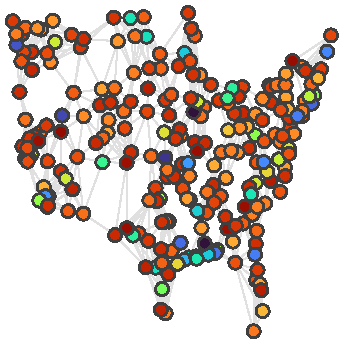
\includegraphics[width=0.15\textwidth]{images/conus_square_signal_1_true.pdf}
}
\sbox{\targetpanelbox}{
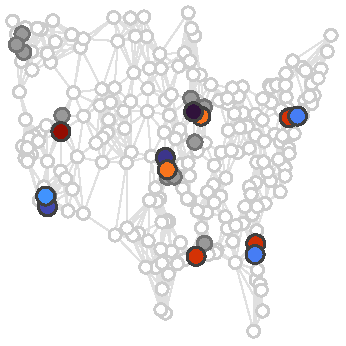
\includegraphics[width=0.15\textwidth]{images/pairwise_top10pct_error_1_true_signal.pdf}
}
\begin{tabular}{@{}cccccc@{\hspace{2pt}}c@{}}
\usebox{\fullpanelbox} &
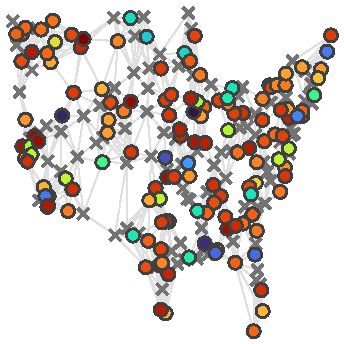
\includegraphics[width=0.15\textwidth]{images/conus_square_signal_2_observed.pdf} &
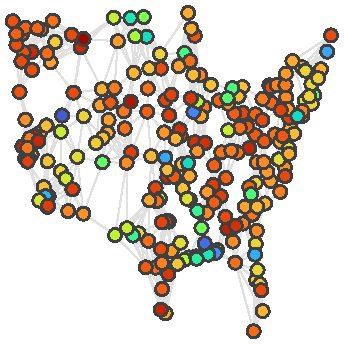
\includegraphics[width=0.15\textwidth]{images/conus_square_signal_3_glr.pdf} &
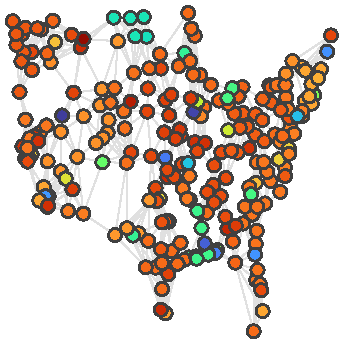
\includegraphics[width=0.15\textwidth]{images/conus_square_signal_4_gtv.pdf} &
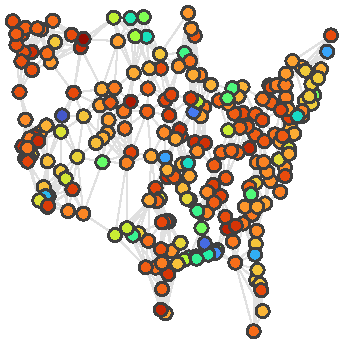
\includegraphics[width=0.15\textwidth]{images/conus_square_signal_5_glr_gtv.pdf} &
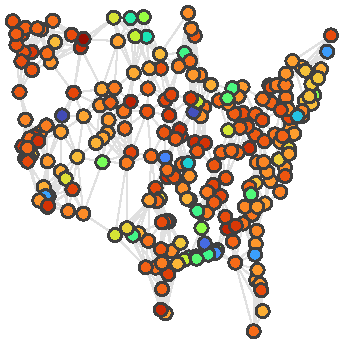
\includegraphics[width=0.15\textwidth]{images/conus_square_signal_6_proposal2.pdf} &
\makebox[0.035\textwidth][l]{

\includegraphics[
height=\ht\fullpanelbox,
keepaspectratio
]{images/colorbar_astp_signal_value.pdf}
} \\[-0.5mm]
\usebox{\targetpanelbox} &
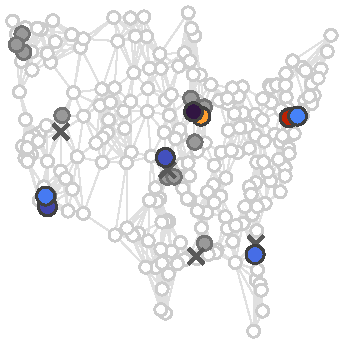
\includegraphics[width=0.15\textwidth]{images/pairwise_top10pct_error_2_observed_signal.pdf} &
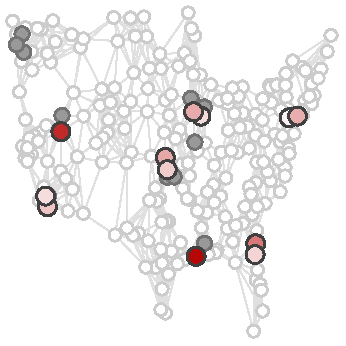
\includegraphics[width=0.15\textwidth]{images/pairwise_top10pct_error_3_glr.pdf} &
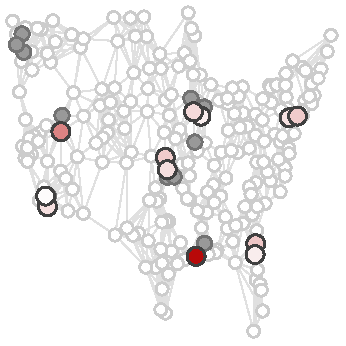
\includegraphics[width=0.15\textwidth]{images/pairwise_top10pct_error_4_gtv.pdf} &
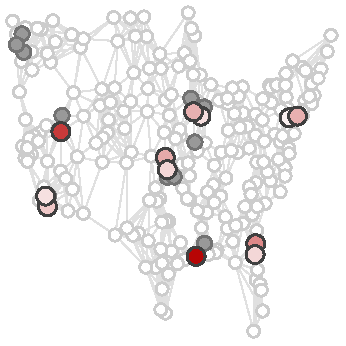
\includegraphics[width=0.15\textwidth]{images/pairwise_top10pct_error_5_glr_gtv.pdf} &
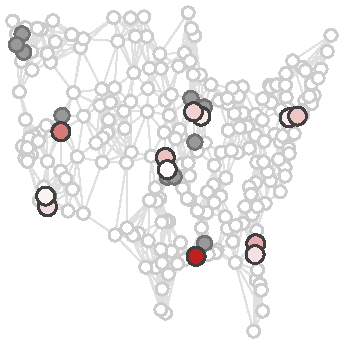
\includegraphics[width=0.15\textwidth]{images/pairwise_top10pct_error_6_proposal2.pdf} &
\makebox[0.035\textwidth][l]{
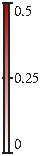
\includegraphics[
height=\ht\targetpanelbox,
keepaspectratio
]{images/colorbar_astp_error.pdf}
} \\[-0.5mm]
\scriptsize\shortstack{True signal\\\phantom{NRMSE = 0.XXXX}} &
\scriptsize\shortstack{Observed signal\\\phantom{NRMSE = 0.XXXX}} &
\scriptsize\shortstack{GLR\\NRMSE = 0.1948} &
\scriptsize\shortstack{GTV\\NRMSE = 0.1865} &
\scriptsize\shortstack{GLR+GTV\\NRMSE = 0.1895} &
\scriptsize\shortstack{Proposed\\NRMSE = \textbf{0.1772}} &
{}
\end{tabular}
\caption{Qualitative station-pressure recovery for a representative daily signal.
The upper row shows the reference, observed, and recovered signals, while the lower row shows the absolute restoration errors at the selected nodes.
Gray nodes and edges indicate the surrounding proxy-graph structure.}
\label{fig:real_world_qualitative}
\end{figure*}

We conduct real-world experiments using meteorological observations from the Global Historical Climatology Network Daily (GHCN-Daily) dataset \cite{Menne2012GHCNDaily} provided by the National Oceanic and Atmospheric Administration (NOAA).
Meteorological observations collected at spatially distributed stations constitute a representative application of graph signal processing, where a graph can naturally be constructed from geographical relationships among the stations.
In practice, however, determining graph-construction parameters that appropriately represent the variation of a target meteorological signal is nontrivial, and a graph constructed solely from geographical proximity does not necessarily capture all factors governing the signal variation.
Moreover, the appropriate spatial relationships can vary across meteorological variables and daily signals.
Consequently, mismatch between the constructed spatial proxy graph and the underlying signal structure can naturally arise even without artificially perturbing the graph.
We use this setting to evaluate the practical effectiveness of the proposed regularizer when graph signal recovery relies on such naturally imperfect spatial proxy graphs.

\subsubsection{Experimental Settings}

We consider daily minimum temperature and station pressure measurements recorded at weather stations in the United States during 2017.
These two meteorological variables are selected as representative spatial signals whose variation cannot necessarily be explained solely by horizontal geographical proximity.
In particular, station pressure can be affected by station elevation as well as horizontal location, making a graph constructed only from inter-station distance a natural example of a potentially imperfect proxy for its variation structure.
For each meteorological variable, the measurements on each day are treated as an underlying graph signal.
Stations without an available measurement for the corresponding variable and day are excluded before graph construction, and 256 stations are randomly selected from the remaining candidates for each daily signal.
The only exception is the station-pressure signal on February 28, 2017, for which only 214 stations with valid measurements are available, resulting in a 214-node graph.
Because the set of available stations can vary across variables and days, the node set and spatial proxy graph are constructed independently for each daily signal.
The same graph-construction procedure is then applied consistently to all daily signals.

For each daily signal, we construct the spatial proxy graph from the geographic locations of the selected stations using a $k$-nearest-neighbor (k-NN) rule, in which each station is connected to its $k$ geographically nearest stations.
We consider $k\in\{4,8\}$ to examine different levels of graph connectivity.
For each connected station pair $(i,j)$, the edge weight is assigned using the Gaussian kernel
$w_{i,j}=\exp(-d_{i,j}^{2}/(2(\eta\bar d)^{2}))$,
where $d_{i,j}$ denotes the geographic distance between the two stations and $\eta\in\{1,2\}$ is the kernel-scale parameter.
The reference distance $\bar d$ is defined as the median of all distances from each station to its first through eighth nearest neighbors.
The four combinations of $k$ and $\eta$ are evaluated as different plausible constructions of the spatial proxy graph, without assuming that any particular construction exactly represents the underlying graph-smoothness structure.

The observation, graph-weight normalization, optimization, and evaluation settings are otherwise the same as those described in Section~V-A.
Following the common parameter-selection protocol in Section~V-A, for each meteorological variable, the aggregation used to select $\tau$ is performed over all daily signals, all four graph-construction settings, and all observation trials.

\subsubsection{Results}

Table~\ref{tab:real_world_results} summarizes the annual-average NRMSEs for the daily minimum-temperature and station-pressure signals under the four spatial proxy-graph constructions.
For each graph-construction setting, the NRMSE is averaged over all daily signals in 2017 and all observation trials.

For the minimum-temperature signals, GLR, GLR+GTV, and the proposed method achieve very similar annual-average NRMSEs across all four graph constructions, whereas GTV yields consistently higher NRMSEs.
The proposed method differs from GLR by at most $0.0002$ in these settings and therefore essentially preserves the recovery performance of GLR for the minimum-temperature signals.

For the station-pressure signals, the proposed method achieves the lowest annual-average NRMSE among all compared methods for all four combinations of $k$ and $\eta$.
In particular, its NRMSE remains lower than those of GLR, GTV, and GLR+GTV regardless of the neighborhood size or Gaussian-kernel scale.
These results indicate that the improvement of the proposed method is not restricted to a particular construction of the spatial proxy graph.

Unlike the synthetic experiments, these real-world experiments do not provide an underlying correct graph or labels specifying which graph relations are inaccurate.
We therefore do not attribute the observed performance differences to a particular type of proxy-graph inaccuracy.
Instead, the results demonstrate the recovery behavior of the compared regularizers when spatial proxy graphs are naturally constructed from geographical relationships under several plausible graph-construction settings.
In particular, station pressure provides a relevant example in which geographical distance alone may not fully represent the signal variation because factors such as station elevation are not explicitly incorporated into the graph.
The consistent performance of the proposed method across the different spatial graph constructions therefore complements the controlled synthetic experiments and supports its practical effectiveness when recovery relies on naturally imperfect proxy graphs.

To complement the annual-average NRMSE evaluation, Fig.~\ref{fig:real_world_qualitative} presents a qualitative comparison for a representative daily station-pressure signal.
The figure shows the underlying signal, the incomplete noisy observations, and the signals recovered by GLR, GTV, GLR+GTV, and the proposed method using the same spatial proxy graph and a common color scale.
In this example, the proposed method achieves the lowest NRMSE of $0.1772$ among the compared methods, and the lower panels show smaller restoration errors at several of the selected nodes.
This qualitative comparison illustrates how the differences among the regularizers appear in the recovered spatial signal and complements the aggregate results reported in Table~\ref{tab:real_world_results}.